

\actTitle{Worksheet 4.2B}



\noindent \textbf{Instructions:}  Work together in groups of  3 or 4 to complete the following problems.\\


\begin{enumerate}


\item $P(x,y)$ on the unit circle corresponding to the real number $t$ is $(5/6,-\sqrt{11}/6)$. 

\begin{enumerate}
\item Make a diagram of the unit circle with $P$ on it. \vfill

\item Determine the values of the six trig functions for $t$. 

\begin{tabular}{l l l }
$\sin(t)=$\phantom{sldkfjdlkdlkjfl}&  $\cos(t)=$\phantom{sldkfjdlkdlkjfl}& $\tan(t)=$\phantom{sldkfjdlkdlkjfl}    \\
& & \\
& & \\
$\csc(t)=$ &  $\sec(t)=$   & $\cot(t)=$    \\
& & \\

\end{tabular}\\


\item Determine $\cos(-t)$ and $\sin(-t)$. \\[1in]

\item Determine $\sin(t+2\pi)$ and $\cos(t+2\pi)$. \\[1in]

\end{enumerate}

\newpage

\item $P(x,y) = (4/5, 3/5)$ corresponds to a real number $t$. 
\begin{enumerate}
\item Make a diagram of the unit circle with $P$ on it. \\[1in]

\item Determine $\cos(t)$ and $\sin(t)$. \\[.5in]

\item Determine $\cos(t+4\pi)$ and $\sin(t-6\pi)$. \\[1in]

\item Determine $\cos(-t)$ and $\sin(-t)$ . \\[1in]

\item Determine $\cos(-t-4\pi)$ and $\sin(-t+100\pi)$. \\[1in]
\end{enumerate}


\newpage

\item Given $\cot(t)=\frac{45}{28}$ for $\pi<t<\frac{3\pi}{2}$.  Use an appropriate Pythagorean identity to find the value of $\csc(t)$

\vfill
\item Write $\tan(t)$ in terms of $\sec(t)$ for
\begin{enumerate}
\begin{multicols}{2}
\item $t$ in Quadrant 2.

\columnbreak
\item $t$ in Quadrant 4.
\end{multicols}
\end{enumerate}

\vfill

\newpage

\item Use the periodic properties of the trigonometric functions to simplify each expression to a \textbf{single} function of $t$.

\begin{enumerate} 
\item $\sin(t+2\pi)\cdot \cot(t+\pi)$\vfill
\item  $\sin(t+2\pi)\cdot \sec(t+2\pi)$\vfill
\end{enumerate}



\item Use the even-odd and periodic properties of the trigonometric functions to simplify.
\begin{enumerate}
\item $\csc(t)-4\csc(-t)$\vfill
\item $-2\sin(3t+2\pi)-3\sin(-3t)$\vfill
\end{enumerate}

\vfill


\item Simplify using properties of trigonometric functions. $$\sin^2(t+2\pi)+\cos^2(t)+\tan^2(t+\pi)$$
\vfill

\newpage
\item Identify values $t$ on the interval $[0,2\pi]$ that make the given function undefined (if any).
\begin{enumerate}
\begin{multicols}{2}
\item $y=\sin(t)$\\[.3in]
\item $y=\cot(t)$\\[.3in]
\item $y=\cos(t)$\\[.3in]
\columnbreak
\item $y=\tan(t)$\\[.3in]
\item $y=\csc(t)$\\[.3in]
\item $y=\sec(t)$\\[.3in]
\end{multicols}
\end{enumerate}

\item Write down all trig functions for which each property applies.
\begin{enumerate}
\item The function is even.\vfill
\item The function is odd.\vfill
\item The period is $2\pi$.\vfill
\item The period is $\pi$.\vfill
\item The domain is all real numbers.\vfill
\item The domain is all real numbers excluding odd multiples of $\frac{\pi}{2}$.\vfill
\item The domain is all real numbers excluding multiples of $\pi$.\vfill
\end{enumerate}
\newpage

\item If you plan on using the unit circle instead of special triangles and the chart for angles on the $x$ and $y$ axes, start memorizing the angles of the unit circle in radians as well as the points along the unit circle.\\
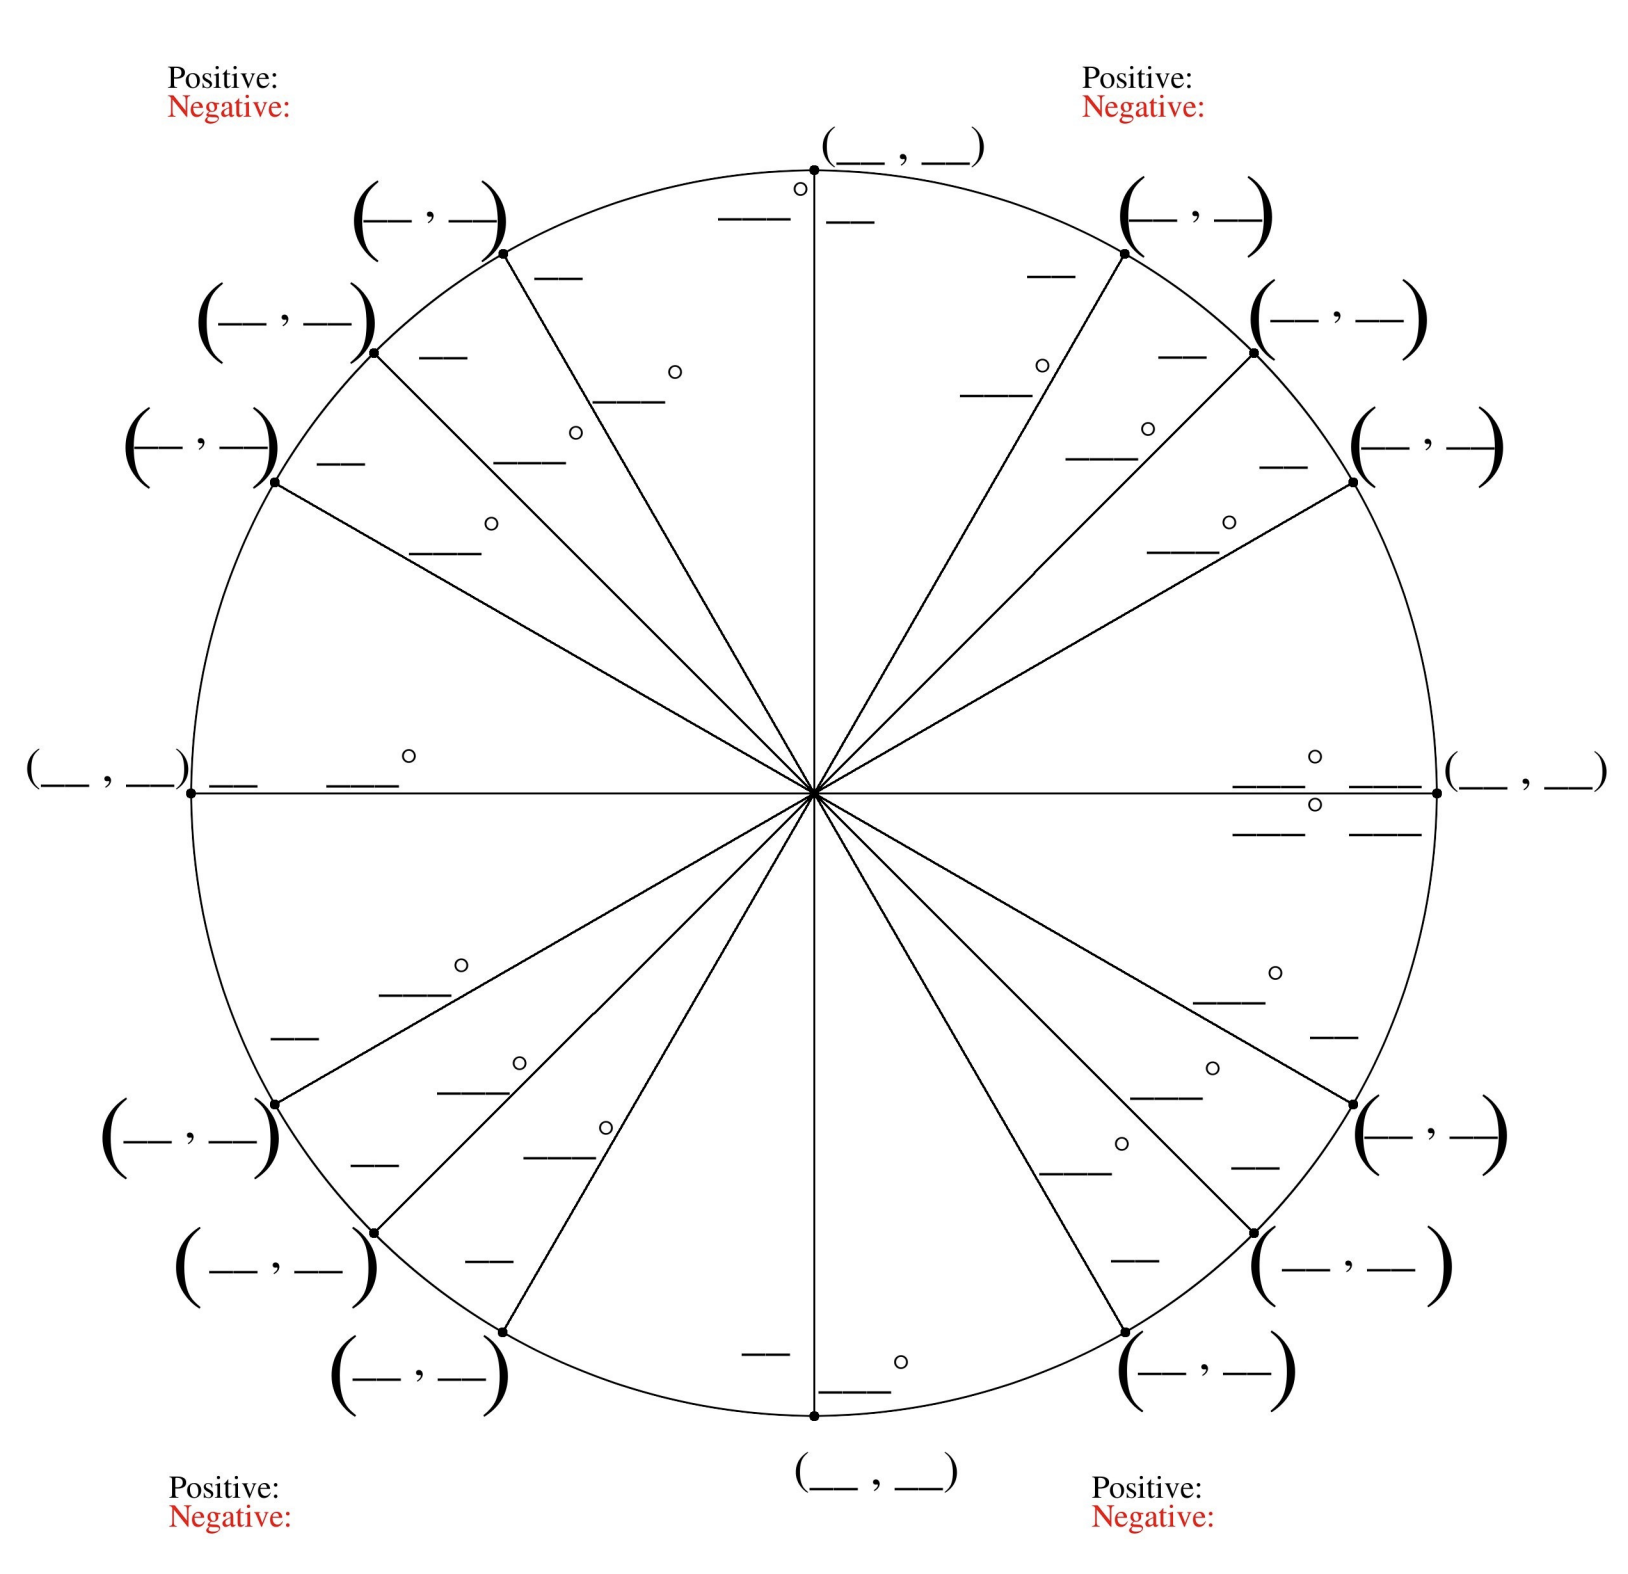
\includegraphics[scale=.6]{blankunitcircle}
\end{enumerate}

